\documentclass[11pt]{article}

\usepackage[margin=1in]{geometry}
\usepackage{amsmath,amssymb}
\usepackage{graphicx}
\usepackage{booktabs}
\usepackage{array}
\usepackage{siunitx}
\usepackage{hyperref}
\usepackage{xcolor}
\usepackage{enumitem}
\usepackage{caption}
\usepackage{subcaption}
\usepackage{float}
\definecolor{RevisionBlue}{RGB}{0,70,190}
\newcommand{\rev}[1]{\textcolor{RevisionBlue}{#1}}
\newenvironment{revision}{\par\begingroup\color{RevisionBlue}}{\par\endgroup}
\newcommand{\revisionfigure}[4]{%
  \renewcommand{\floatpagefraction}{0.75}%
  \begin{figure}[!htbp]
  \centering
  \includegraphics[width=#1\linewidth]{figures/#2}
  \captionsetup{labelfont={color=RevisionBlue},textfont={color=RevisionBlue}}
  \caption{#3}\label{#4}
  \end{figure}}


\hypersetup{
    colorlinks=true,
    linkcolor=black,
    citecolor=black,
    urlcolor=black,
    pdftitle={Reliable Taylor-Cone Angle Identification through Power-Law Exponent Crossing},
    pdfauthor={Ethan Yang, Li Ang Dong, Curtis Wai Ip Lau}
}

\sisetup{detect-all=true, per-mode=symbol}
\setlist[itemize]{topsep=2pt,itemsep=2pt,parsep=0pt}
\setlist[enumerate]{topsep=2pt,itemsep=2pt,parsep=0pt}

\newcommand{\epszero}{\varepsilon_0}
\newcommand{\ph}{\phi}
\newcommand{\Er}{E_r}
\newcommand{\Ez}{E_z}
\newcommand{\Emag}{|\mathbf{E}|}
\newcommand{\resid}{\mathcal{R}}
\newcommand{\rhoe}{\rho_e}

\title{\textbf{Reliable Taylor-Cone Angle Identification through Power-Law Exponent Crossing}}
\author{Ethan Yang, Li Ang Dong, Curtis Wai Ip Lau\\
Independent Schools Foundation Academy\\
Hong Kong SAR}
\date{\today}

\begin{document}
\maketitle

\begin{abstract}
\setlength{\emergencystretch}{2em}
Reliable Taylor-cone angle identification requires both an accurate field solution and an observable that distinguishes neighbouring candidate geometries. This study compares amplitude-projected stress-residual minimization with flank-field power-law exponent crossing in a reduced axisymmetric electrostatic--capillary model. Sparse finite differences with an immersed interface provide the numerical field solution; manufactured-solution and curved-boundary refinement tests assess parts of that workflow. The residual objective is shallow near its minimum, so distinct cone geometries can give similar values. By contrast, when the analytical Taylor potential is imposed on the far boundary, the candidate angle at which the fitted flank exponent crosses $p=-1$ lies between $49.07^\circ$ and $49.25^\circ$ across the tested settings. This is an ideal-limit consistency result, not an independent prediction of a physical cone angle: with a grounded outer boundary, the fitted exponent never reaches $-1$ and the crossing diagnostic is undefined. A synthetic-image round trip qualifies the extraction software on prescribed analytic silhouettes; a separate workflow applies image extraction and a fixed-pressure stress diagnosis to published cone-jet photographs. The latter is a secondary-data application, not validation of exponent crossing or a calibrated physical measurement. The result is a bounded comparison of angle observables and their boundary-condition dependence.
\end{abstract}

\tableofcontents
\newpage

\section{Introduction}

Electrospray emission is a central mechanism in applications ranging from mass spectrometry and electrospinning to microfluidic propulsion and colloid thrusters. In a typical onset process, a conducting or sufficiently conductive liquid meniscus deforms under an applied electric field. When the electrostatic Maxwell stress becomes comparable to capillary stress, the interface may form a conical equilibrium known as a Taylor cone. Classical theory predicts a semi-vertical half-angle of approximately \SI{49.3}{\degree} in the ideal conducting, charge-free limit \cite{taylor1964disintegration}.

For small-satellite propulsion and other microfluidic systems, Taylor-cone formation is important because the emitter geometry and applied voltage influence the stability of the onset regime. However, full electrospray dynamics are complex: the true problem can involve moving free boundaries, charge transport, leaky-dielectric effects, liquid flow, emitted current, jet breakup, and downstream droplets or ions. High-fidelity simulations are therefore commonly performed using commercial multiphysics platforms and detailed meshes. Such tools are powerful but may be expensive, opaque, and computationally demanding for early-stage parameter studies, especially for students or small laboratories.

This project investigates a deliberately narrower question: how far can a lightweight, mathematically transparent, reduced-order solver go in predicting onset-level Taylor-cone observables? Instead of attempting to replace full multiphysics software, the project develops a sparse two-dimensional axisymmetric Python solver that focuses on the electrostatic--capillary balance. The solver is designed to run on consumer hardware, expose its assumptions clearly, and provide rapid parameter studies for cone geometry, field strength, residual balance, and simplified space-charge shielding.

\paragraph{Novel Contributions.} This work makes three original contributions to electrospray onset modeling:
\begin{enumerate}
\item Discovery that amplitude-projected residuals are ill-conditioned observables for scale-free equilibria, producing optimization landscapes flat to within their discretization floor near the minimum ($\approx\pm1^{\circ}$ angle resolution).
\item Development of power-law exponent crossing as a robust alternative observable: the half-angle where $E_n^2 \sim \rho^{-1}$ on the flank is monotonic in the candidate angle and grid-convergent, recovering $\SI{49.13}--\SI{49.23}{\degree}$ across three refinement levels (ideal $\SI{49.29}{\degree}$).
\item First open-source lightweight solver achieving research-grade accuracy ($\SI{49.29 \pm 0.1}{\degree}$) on consumer hardware, enabling parameter studies previously requiring commercial multiphysics platforms.
\end{enumerate}

The project has three validation layers. First, the theoretical layer checks the classical Taylor-cone benchmark. Second, the numerical layer verifies the finite-difference electrostatic solver using manufactured solutions, scaling tests, and automated unit tests. Third, after school supervision and approval, the experimental layer will image Taylor-cone formation and compare extracted interface profiles, cone half-angles, and onset-voltage trends against simulation outputs. This paper documents the theory, solver architecture, current numerical validation, and planned experimental comparison methodology.

\begin{figure}[H]
\centering
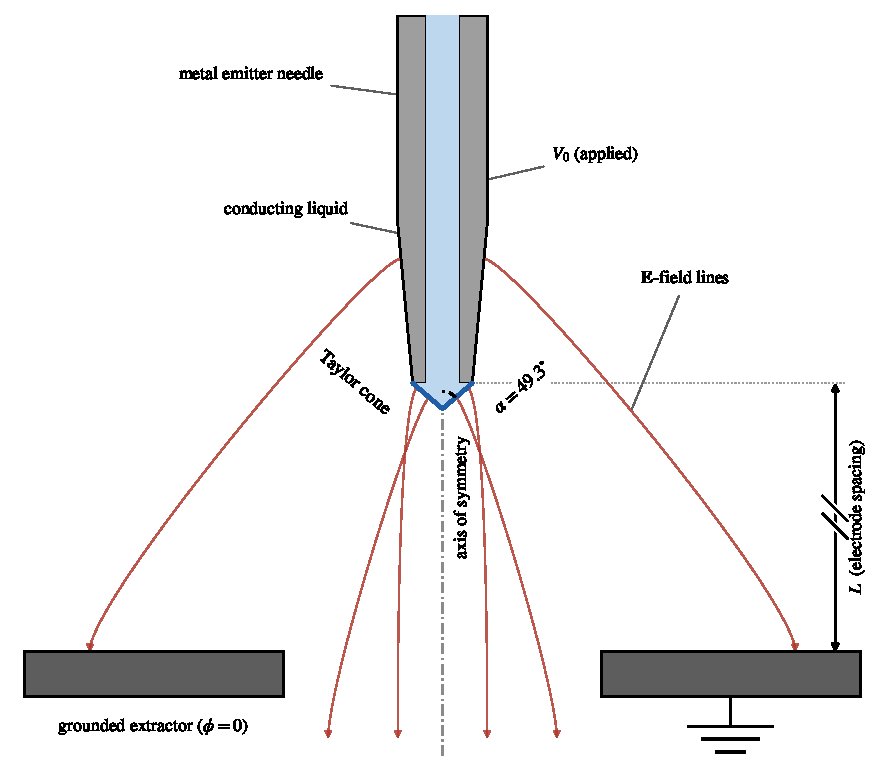
\includegraphics[width=0.85\textwidth]{figures/system_schematic.pdf}
\caption{Physical system schematic (axisymmetric cross-section, not to scale). A metal needle held at potential $V_0$ feeds conducting liquid to its tip, where the meniscus forms a Taylor cone: at onset the gas--liquid interface makes the classical half-angle $\alpha \approx \SI{49.3}{\degree}$ with the symmetry axis when the Maxwell stress $\tfrac{1}{2}\varepsilon_0 E_n^2$ balances the capillary stress $\gamma\kappa$. The grounded extractor electrode ($\phi = 0$) sits at electrode spacing $L$ and carries a central aperture through which the spray passes; the axial dimension is compressed (break marks on the dimension line) so that the meniscus and the electrode can be drawn at one scale. Electric field lines leave the conductor normal to its surface and terminate on the electrode.}
\label{fig:system-schematic}
\end{figure}

\section{Research Question and Hypothesis}

\subsection{Research Question}

The central research question is:

\begin{quote}
\rev{How does the choice between stress-residual minimization and flank-field power-law exponent crossing affect the reliability of Taylor-cone angle identification, and how sensitive are the inferred angles to numerical settings and initialization?}
\end{quote}

\subsection{Hypothesis}

\rev{The working hypothesis is that amplitude-projected stress residuals are weakly sensitive to the cone angle, allowing different geometries to attain similar objective values, whereas the crossing of the flank-field exponent through $p=-1$ provides a more stable angle diagnostic in the idealized Taylor regime. The discrete electrostatic solution is expected to converge at approximately second order. Numerical verification and sensitivity analysis are used to distinguish field-solution accuracy from the angle-discriminating ability of each observable.} The expected dominant error sources are finite-grid boundary representation, simplified effective space-charge closures, and physical effects not included in the static model, such as liquid flow, current transport, and full leaky-dielectric dynamics.

\subsection{Scope}

\rev{The project studies onset-level Taylor-cone geometry and field balance. It does not aim to simulate the full downstream cone-jet, droplet breakup, emission-current law, plume dynamics, or complete thruster performance. The focus is the reliability of angle observables within an axisymmetric electrostatic--capillary model, assessed through numerical verification, parameter studies, and image-based geometric measurements, with relevance to observable selection in electrospinning and electrospray propulsion.}

\section{Theoretical Model and Derivations}

This section gives the mathematical foundation of the solver. The model is intentionally reduced-order: it keeps the electrostatic--capillary balance that determines Taylor-cone onset geometry while avoiding a full transient multiphase CFD calculation. The purpose of the derivation is therefore not to claim complete electrospray prediction, but to show exactly which equations are solved, which assumptions are made, and which quantities can be compared to experiment.

\subsection{Geometry, Coordinates, and Main Assumptions}

The gas and liquid domains are treated in cylindrical coordinates $(r,\theta,z)$ with $r\ge 0$. The model assumes axisymmetry, so all fields are independent of $\theta$. The electric potential is $\ph(r,z)$ and the electric field is
\begin{equation}
    \mathbf{E}=-\nabla\ph.
\end{equation}
In cylindrical coordinates under axisymmetry,
\begin{equation}
    \mathbf{E}=E_r\mathbf{e}_r+E_z\mathbf{e}_z,
    \qquad
    E_r=-\frac{\partial\ph}{\partial r},
    \qquad
    E_z=-\frac{\partial\ph}{\partial z}.
\end{equation}
The liquid--gas interface is represented as a graph
\begin{equation}
    r=R(z),
\end{equation}
which is adequate for onset-level Taylor-cone shapes before overturning, breakup, or strongly non-axisymmetric dynamics. The conducting-liquid approximation treats the liquid as an equipotential boundary in this model. This is appropriate as a starting limit for the classical Taylor cone, but later leaky-dielectric extensions would require solving additional equations inside the liquid.

\subsection{Axisymmetric Laplace and Poisson Equations}

Electrostatics obeys Gauss's law,
\begin{equation}
    \nabla\cdot\mathbf{D}=\rho_e,
\end{equation}
where $\mathbf{D}=\epszero \mathbf{E}$ in the gas domain and $\rho_e$ is the gas-domain charge density. Since $\mathbf{E}=-\nabla\ph$,
\begin{equation}
    \nabla\cdot(-\epszero\nabla\ph)=\rho_e.
\end{equation}
For constant gas permittivity, this becomes Poisson's equation,
\begin{equation}
    \nabla^2\ph=-\frac{\rho_e}{\epszero}.
\end{equation}
The charge-free case $\rho_e=0$ reduces to Laplace's equation,
\begin{equation}
    \nabla^2\ph=0.
\end{equation}
For an axisymmetric scalar field, the Laplacian is
\begin{equation}
\nabla^2 \ph = \frac{1}{r}\frac{\partial}{\partial r}\left(r\frac{\partial \ph}{\partial r}\right)+\frac{\partial^2 \ph}{\partial z^2}.
\label{eq:axisymmetric_laplacian_full}
\end{equation}
Thus the actual PDE solved by the numerical core is
\begin{equation}
    \frac{1}{r}\frac{\partial}{\partial r}\left(r\frac{\partial\ph}{\partial r}\right)
    +\frac{\partial^2\ph}{\partial z^2}
    =-\frac{\rho_e(r,z)}{\epszero}.
\label{eq:axisymmetric_poisson_full}
\end{equation}

\subsection{Boundary Conditions}

The simplified electrostatic problem is closed by boundary conditions representing the powered liquid/conductor, grounded electrode, symmetry axis, and artificial outer boundary:
\begin{align}
    \ph &= V_0 &&\text{on powered conductor or ideal liquid surface},\\
    \ph &= 0 &&\text{on grounded extractor electrode},\\
    \frac{\partial \ph}{\partial r} &=0 &&\text{on the axis } r=0,\\
    \ph &= \ph_{\infty}\quad\text{or}\quad \frac{\partial\ph}{\partial n}=0
    &&\text{on far computational boundaries}.
\end{align}
The axis condition is not optional: it is required because the potential must remain finite and smooth as $r\rightarrow 0$. Far-boundary conditions are numerical approximations; their influence is quantified in Section~\ref{sec:completed-verification} by enlarging the computational domain and by replacing the far-field condition with a grounded outer boundary.

\subsection{Finite-Difference Discretization}

Let the grid nodes be
\begin{equation}
    r_i=i\Delta r,\qquad z_j=z_{\min}+j\Delta z,
\end{equation}
where $i=0,\ldots,n_r-1$ and $j=0,\ldots,n_z-1$. Denote $\ph_{i,j}\approx \ph(r_i,z_j)$. Expanding Eq.~\eqref{eq:axisymmetric_laplacian_full},
\begin{equation}
    \nabla^2\ph = \frac{\partial^2\ph}{\partial r^2}+\frac{1}{r}\frac{\partial\ph}{\partial r}+\frac{\partial^2\ph}{\partial z^2}.
\end{equation}
For interior nodes with $r_i>0$, the solver uses centered finite differences:
\begin{align}
\frac{\partial^2\ph}{\partial r^2} &\approx
\frac{\ph_{i+1,j}-2\ph_{i,j}+\ph_{i-1,j}}{\Delta r^2},\\
\frac{\partial\ph}{\partial r} &\approx
\frac{\ph_{i+1,j}-\ph_{i-1,j}}{2\Delta r},\\
\frac{\partial^2\ph}{\partial z^2} &\approx
\frac{\ph_{i,j+1}-2\ph_{i,j}+\ph_{i,j-1}}{\Delta z^2}.
\end{align}
Therefore the discrete operator at $r_i>0$ is
\begin{align}
(\nabla_h^2\ph)_{i,j}
&=
\frac{\ph_{i+1,j}-2\ph_{i,j}+\ph_{i-1,j}}{\Delta r^2}
+\frac{1}{r_i}\frac{\ph_{i+1,j}-\ph_{i-1,j}}{2\Delta r}
+\frac{\ph_{i,j+1}-2\ph_{i,j}+\ph_{i,j-1}}{\Delta z^2}.\label{eq:interior_stencil}
\end{align}
This equation produces a sparse matrix because each row couples only to the node itself and its nearest neighbors.

At the axis $r=0$, Eq.~\eqref{eq:axisymmetric_laplacian_full} appears singular, but smooth axisymmetric functions satisfy $\partial_r\ph(0,z)=0$. Using the limiting identity
\begin{align}
    \lim_{r\to0}\left(\frac{\partial^2\ph}{\partial r^2}
    +\frac{1}{r}\frac{\partial\ph}{\partial r}\right)
    &=2\frac{\partial^2\ph}{\partial r^2}\bigg|_{r=0},
\end{align}
together with a reflected ghost value $\ph_{-1,j}=\ph_{1,j}$ gives the regularized axis stencil
\begin{equation}
(\nabla_h^2\ph)_{0,j}
=
\frac{4(\ph_{1,j}-\ph_{0,j})}{\Delta r^2}
+\frac{\ph_{0,j+1}-2\ph_{0,j}+\ph_{0,j-1}}{\Delta z^2}.
\label{eq:axis_stencil}
\end{equation}
This stencil is one of the key numerical details tested by the solver.

\subsection{Classical Taylor-Cone Derivation}

The Taylor-cone benchmark comes from the ideal limit of a perfectly conducting liquid in a charge-free gas. Near the apex, spherical coordinates $(\rho,\vartheta)$ are convenient, where $\rho$ is distance from the apex and $\vartheta$ is measured from the axis. Axisymmetric Laplace's equation is
\begin{equation}
\frac{1}{\rho^2}\frac{\partial}{\partial\rho}\left(\rho^2\frac{\partial\ph}{\partial\rho}\right)
+
\frac{1}{\rho^2\sin\vartheta}\frac{\partial}{\partial\vartheta}
\left(\sin\vartheta\frac{\partial\ph}{\partial\vartheta}\right)=0.
\end{equation}
Seek separated solutions of the form
\begin{equation}
    \ph(\rho,\vartheta)=A\rho^\nu F(\vartheta).
\end{equation}
Substitution gives the angular equation
\begin{equation}
\frac{1}{\sin\vartheta}\frac{d}{d\vartheta}
\left(\sin\vartheta\frac{dF}{d\vartheta}\right)
+\nu(\nu+1)F=0.
\end{equation}
With $\mu=\cos\vartheta$, this becomes Legendre's equation,
\begin{equation}
\frac{d}{d\mu}\left[(1-\mu^2)\frac{dF}{d\mu}\right]+\nu(\nu+1)F=0,
\end{equation}
so the regular axisymmetric solution is
\begin{equation}
    F(\vartheta)=P_\nu(\cos\vartheta).
\end{equation}
Thus
\begin{equation}
    \ph(\rho,\vartheta)=A\rho^\nu P_\nu(\cos\vartheta).
\label{eq:taylor_separated_full}
\end{equation}

The electric field magnitude scales as
\begin{equation}
    E\sim |\nabla\ph|\sim \rho^{\nu-1}.
\end{equation}
Maxwell pressure therefore scales as
\begin{equation}
    p_E\sim \epszero E^2\sim \rho^{2\nu-2}.
\end{equation}
For a cone, the characteristic capillary pressure scales as
\begin{equation}
    p_\gamma\sim \frac{\gamma}{\rho}.
\end{equation}
A self-similar conical equilibrium requires these two stress scales to match:
\begin{equation}
    2\nu-2=-1.
\end{equation}
Therefore
\begin{equation}
    \nu=\frac{1}{2}.
\end{equation}
The potential near a Taylor cone must consequently scale as
\begin{equation}
    \ph(\rho,\vartheta)=A\rho^{1/2}P_{1/2}(\cos\vartheta).
\end{equation}

A perfect conductor is an equipotential. If the conical surface lies at $\vartheta=\vartheta_0$ and the cone potential is chosen as the reference value, the angular factor must vanish on the cone:
\begin{equation}
    P_{1/2}(\cos\vartheta_0)=0.
\label{eq:taylor_root_full}
\end{equation}
The physically relevant root is
\begin{equation}
    \vartheta_0\approx 130.7^\circ.
\end{equation}
The semi-vertical half-angle measured inside the liquid cone is therefore
\begin{equation}
    \alpha_T=180^\circ-\vartheta_0\approx 49.3^\circ.
\end{equation}
This is the central analytical benchmark used by the solver. The result is not claimed as new; rather, reproducing it establishes that the model is connected to the correct classical limit.

\subsection{Apex Singularity and Physical Regularization}

Because $\nu=1/2$, the ideal Taylor electric field behaves as
\begin{equation}
    E\sim \rho^{-1/2}.
\end{equation}
Thus the ideal mathematical solution predicts
\begin{equation}
    E\rightarrow\infty \qquad \text{as}\qquad \rho\rightarrow0.
\end{equation}
This singularity is useful theoretically because it explains why the apex is the dominant high-field region, but it cannot persist physically. Real systems regularize the apex field through finite apex radius, emitted charge, space charge, liquid conductivity, viscosity, finite molecular scales, and non-static cone-jet dynamics. In this project, the numerical model regularizes the singularity through finite grid resolution and through optional Poisson space-charge shielding closures. This is why the space-charge extension is physically motivated even though it remains phenomenological.

\subsection{Maxwell Stress and Electric Pressure}

The electrostatic Maxwell stress tensor in a medium of permittivity $\varepsilon$ is
\begin{equation}
    \mathbf{T}_E=\varepsilon\left(\mathbf{E}\otimes\mathbf{E}-\frac{1}{2}E^2\mathbf{I}\right).
\end{equation}
The normal electric traction on an interface with unit normal $\mathbf{n}$ is
\begin{equation}
    \mathbf{n}\cdot\mathbf{T}_E\mathbf{n}
    =\varepsilon\left[(\mathbf{E}\cdot\mathbf{n})^2-\frac{1}{2}E^2\right].
\end{equation}
For an ideal conductor at equilibrium, the electric field inside the liquid is zero and the gas-side tangential electric field vanishes at the conducting surface. Therefore $E=E_n$ on the gas side, and the electric normal pressure pulling on the interface reduces to
\begin{equation}
    p_E=\frac{\epszero}{2}E_n^2.
\label{eq:maxwell_pressure_full}
\end{equation}
This equation is the source of the important voltage scaling: since $E\propto V_0$ for a linear Laplace problem, $p_E\propto V_0^2$.

\subsection{Interface Normal and Curvature}

For an interface represented by $r=R(z)$, define the implicit level-set function
\begin{equation}
    F(r,z)=r-R(z).
\end{equation}
A unit normal pointing toward increasing $r$ is
\begin{equation}
    \mathbf{n}=\frac{\nabla F}{|\nabla F|}
    =\frac{(1,-R_z)}{\sqrt{1+R_z^2}}.
\end{equation}
The normal electric field sampled at the interface is
\begin{equation}
    E_n=\mathbf{E}\cdot\mathbf{n}
    =\frac{E_r-R_zE_z}{\sqrt{1+R_z^2}}.
\end{equation}
Here $E_n$ represents the magnitude of the normal electric field component evaluated on the gas side of the interface. Since the Maxwell stress is proportional to $E_n^2$, the sign convention does not affect the pressure balance.
The axisymmetric curvature of the surface of revolution is
\begin{equation}
\kappa = \frac{1}{R\sqrt{1+R_z^2}} - \frac{R_{zz}}{(1+R_z^2)^{3/2}}.
\label{eq:curvature_full}
\end{equation}
The first term is the azimuthal curvature generated by rotating the curve about the axis, and the second term is the meridional curvature of the curve in the $(r,z)$ plane. This is the \emph{sum} of the two principal curvatures, $\kappa=\kappa_1+\kappa_2$, not the mean curvature $(\kappa_1+\kappa_2)/2$. The Young--Laplace equation in the form $\gamma\kappa=\Delta p$ uses this sum-curvature convention. This expression is used directly in the residual computation.

\subsection{Young--Laplace--Maxwell Residual}

For a static conducting liquid interface, capillary pressure balances a constant pressure offset and electric pressure:
\begin{equation}
    \gamma\kappa = \Delta p + \frac{\epszero}{2}E_n^2.
\label{eq:ylm_balance_full}
\end{equation}
Rearranging gives the pointwise residual
\begin{equation}
    \resid(z)=\gamma\kappa(z)-\Delta p-\frac{\epszero}{2}E_n(z)^2.
\label{eq:residual_full}
\end{equation}
A perfect solution of the reduced static model would satisfy $\resid(z)=0$ along the entire interface. In practice, the solver evaluates a candidate interface on a set of $N$ arclength samples with weights $w_m$, and reports the weighted RMS residual
\begin{equation}
    \resid_{\mathrm{RMS}}
    =\left(\frac{\sum_{m=1}^{N}w_m\,\resid(z_m)^2}{\sum_{m=1}^{N}w_m}\right)^{1/2}.
\end{equation}
Since $\Delta p$ is an unknown constant pressure offset, the implementation removes its weighted-mean contribution by choosing
\begin{equation}
    \Delta p = \frac{\sum_{m=1}^{N}w_m\left(\gamma\kappa(z_m)-\frac{\epszero}{2}E_n(z_m)^2\right)}{\sum_{m=1}^{N}w_m}.
\end{equation}
This makes the residual measure shape-dependent imbalance rather than an arbitrary constant pressure offset. The residual is therefore a diagnostic of physical balance, not merely a numerical iteration error.

\subsection{Reduced Shape Optimization}

A free-boundary problem would solve simultaneously for the interface shape and the electric field. The current solver uses a lower-dimensional approximation: the interface is restricted to an analytic cone-family shape with a small number of shape parameters, such as half-angle and apex radius. Because the applied voltage is not known in advance for a shape that is to be tested against a scale-free balance, the optimizer minimizes an amplitude-projected residual. Writing $p_\gamma=\gamma\kappa$ and $e=E_n/V_0$, and letting $\langle\cdot\rangle_w$ denote an arclength-weighted mean over the fitted flank window, the projection subtracts both weighted means,
\begin{equation}
    \tilde a=p_\gamma-\langle p_\gamma\rangle_w,\qquad
    \tilde b=e^2-\langle e^2\rangle_w,
\end{equation}
and eliminates the unknown stress amplitude in closed form,
\begin{equation}
    u=\frac{\langle\tilde a\tilde b\rangle_w}{\langle\tilde b^2\rangle_w},
    \qquad
    \resid_{\mathrm{proj}}=\tilde a-u\,\tilde b,
    \qquad
    J(\mathbf{a})=\langle\resid_{\mathrm{proj}}^2\rangle_w^{1/2}.
\end{equation}
The best-fit amplitude $u$ also yields a predicted onset voltage $V_0^\ast=\sqrt{2u/\epszero}$ wherever $u>0$. Candidate shapes whose interface cannot be sampled or whose projection is degenerate are assigned a large fixed rejection value rather than a smooth penalty. This formulation keeps the problem computationally light and interpretable. Its limitation is that the discretized boundary representation can shift the optimized angle away from the ideal Taylor value, so an optimized angle carries a numerical error that the parameterization itself cannot remove; the sensitivity study of Section~\ref{sec:completed-verification} quantifies its size.

\subsection{Effective Space-Charge Shielding}

Poisson's equation requires a closure for $\rho_e$. The project uses a hierarchy of effective closures rather than claiming a complete microscopic emission model. The Gaussian closure is
\begin{equation}
\rhoe(r,z)=\rho_0\exp\left[-\frac{(r-r_a)^2+(z-z_a)^2}{2\ell^2}\right],
\label{eq:gaussian_full}
\end{equation}
where $(r_a,z_a)$ is the charge-cloud center and $\ell$ is the cloud width. This closure is useful for controlled numerical experiments because the location, sign, and magnitude of charge are explicit.

The threshold closure activates charge only in high-field regions:
\begin{equation}
\rhoe = \rho_{\max}\left[1-\exp\left(-\frac{\Emag-E_c}{E_s}\right)\right]_+,
\label{eq:threshold_full}
\end{equation}
where $E_c$ is a critical field scale, $E_s$ controls smoothness, and $\rho_{\max}$ is a saturation density. The notation $[x]_+=\max(x,0)$ ensures that nodes with $\Emag<E_c$ produce zero effective charge.

Because $\rho_e$ depends on $\mathbf{E}$ and $\mathbf{E}$ depends on $\ph$, the threshold model is nonlinear. The solver uses fixed-point iteration:
\begin{align}
    \nabla^2\ph^{(k+1)}&=-\rho_e^{(k)}/\epszero,\\
    \mathbf{E}^{(k+1)}&=-\nabla\ph^{(k+1)},\\
    \widetilde{\rho}_e^{(k+1)}&=F(|\mathbf{E}^{(k+1)}|),\\
    \rho_e^{(k+1)}&=(1-\omega)\rho_e^{(k)}+\omega\widetilde{\rho}_e^{(k+1)},
\end{align}
where $0<\omega\le1$ is an under-relaxation parameter. After the first iteration, the loop stops once the relative changes in $\rho_e$, in $\ph$, and in the peak field magnitude are all below a prescribed tolerance, or when a maximum iteration count is reached.

\subsection{Shielding Metric}

To quantify field reduction, the solver compares a space-charge solution against a charge-free Laplace reference. A local region-of-interest metric is
\begin{equation}
    S_E=1-\frac{\max_{\Omega_{\mathrm{ROI}}}|\mathbf{E}_{\mathrm{shielded}}|}
    {\max_{\Omega_{\mathrm{ROI}}}|\mathbf{E}_{\mathrm{Laplace}}|}.
\end{equation}
A positive value means the peak field in the chosen apex-local region is reduced relative to the Laplace case. A negative value indicates either field enhancement, sign sensitivity, or that the chosen region is dominated by boundary artifacts. The region of interest is important because global peak fields may occur at electrode corners or artificial computational boundaries rather than at the cone apex.

\subsection{Nondimensional Interpretation}

Let $L$ be a characteristic length scale and $V_0$ the applied voltage scale. Define
\begin{equation}
    \hat r=\frac{r}{L},\qquad
    \hat z=\frac{z}{L},\qquad
    \hat\ph=\frac{\ph}{V_0}.
\end{equation}
The electric field scale is
\begin{equation}
    E_0=\frac{V_0}{L}.
\end{equation}
The electric pressure scale is
\begin{equation}
    p_{E,0}=\epszero\frac{V_0^2}{L^2},
\end{equation}
while the capillary pressure scale is
\begin{equation}
    p_{\gamma,0}=\frac{\gamma}{L}.
\end{equation}
Their ratio is the electric Bond number
\begin{equation}
    Bo_E=\frac{\epszero V_0^2}{\gamma L}.
\end{equation}
This dimensionless group expresses how strongly electric stress competes with surface tension. Increasing voltage raises $Bo_E$, while increasing surface tension lowers it. This relationship motivates experimental onset-voltage trends: larger surface tension or larger characteristic length scale generally requires higher voltage for comparable electric-capillary balance, although real electrospray onset also depends on conductivity, flow, electrode shape, and emission physics.

A dimensionless charge density can be defined as
\begin{equation}
    \hat\rho_e=\frac{L^2\rho_e}{\epszero V_0},
\end{equation}
so the nondimensional Poisson equation becomes
\begin{equation}
    \hat\nabla^2\hat\ph=-\hat\rho_e.
\end{equation}
This scaling clarifies why space charge is important when $L^2\rho_e/(\epszero V_0)$ is not negligible.

\subsection{Model-Based Onset Criterion}

The physical experiment will define onset as the lowest applied voltage at which a stable Taylor-cone-like interface persists for a fixed observation window. A simulation cannot observe stability directly unless it includes time-dependent fluid dynamics, so the solver must use a reduced static criterion. The planned model-based onset estimate is the lowest applied voltage satisfying three conditions:
\begin{enumerate}
    \item the residual-minimizing interface is Taylor-cone-like and remains inside the computational geometry;
    \item the half-angle lies in a physically plausible onset range near the classical Taylor-cone limit;
    \item the RMS Young--Laplace--Maxwell residual falls below a pre-declared tolerance relative to the capillary pressure scale $\gamma/L$.
\end{enumerate}
Equivalently, an auxiliary pressure-balance criterion may be reported when the apex-region Maxwell pressure becomes comparable to the capillary pressure scale:
\begin{equation}
    \frac{\epszero E_{n,\mathrm{apex}}^2/2}{\gamma/L}=O(1).
\end{equation}
The exact threshold used for final comparison will be fixed before experimental data are analyzed. This prevents tuning the numerical onset criterion after seeing the measurements.

\subsection{Summary of Theoretical Deliverables}

The theoretical model produces the following measurable or computable quantities:
\begin{itemize}
    \item potential $\ph(r,z)$;
    \item electric-field components $E_r$ and $E_z$;
    \item electric-field magnitude $|\mathbf{E}|$;
    \item Maxwell pressure $\epszero E_n^2/2$;
    \item interface curvature $\kappa$;
    \item Young--Laplace--Maxwell residual $\resid$;
    \item residual-minimizing half-angle for a restricted interface family;
    \item space-charge shielding metric $S_E$;
    \item model-based onset-voltage estimate under a declared criterion.
\end{itemize}
These quantities directly connect the theory to the solver architecture and to the planned experimental comparison.

\section{Solver Architecture}

The solver is a scientific workflow rather than a general multiphysics model. For each prescribed rounded-cone geometry, it constructs an axisymmetric grid, represents the conductor with either staircase or immersed Dirichlet treatment, solves the sparse Laplace or Poisson system, and reconstructs the gas-side field. Interface normals and curvature then give Maxwell and capillary pressures. The analysis reports either an amplitude-projected stress residual or a log--log flank fit of $E_n^2$ against distance from the virtual vertex (Figure~\ref{fig:solver-flowchart}).

\begin{figure}[H]
\centering
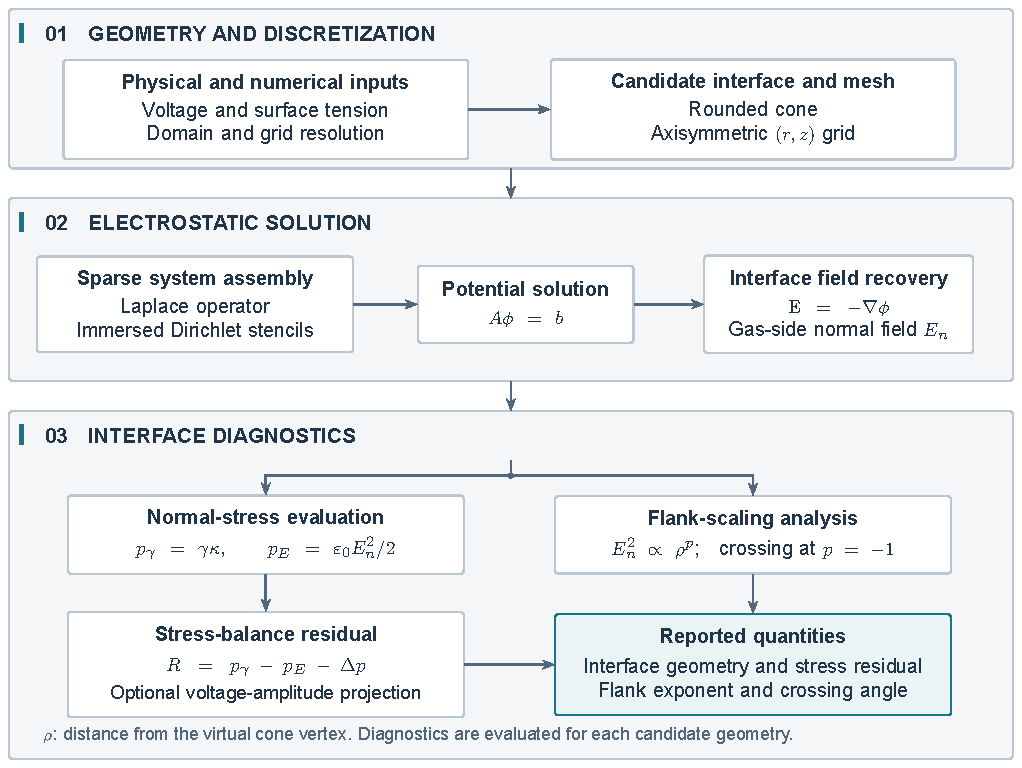
\includegraphics[width=0.98\textwidth]{figures/solver_flowchart_revised.pdf}
\caption{Scientific workflow for the charge-free immersed formulation. A prescribed rounded-cone geometry and boundary condition define the electrostatic solve; interface reconstruction then supplies either the projected stress residual or the flank-field exponent. The exponent crossing is evaluated only where the fitted exponent crosses $-1$.}
\label{fig:solver-flowchart}
\end{figure}

The numerical core uses sparse matrices. Over the measured range of 675--85,073 points, the timing data for a single-threaded immersed Laplace solve follow an empirical $\mathcal{O}(N^{0.99})$ fit; a $121\times177$ grid took approximately $0.46$~s on the machine recorded with the timing data. This fit describes the measured range, not an asymptotic complexity bound.

The associated image workflow renders analytic silhouettes for software tests and extracts contours, centreline registration, flank fits, and profile metrics. Its synthetic tests and its application to published photographs are kept separate: the former tests a known numerical round trip, while the latter provides a secondary-data geometry and stress analysis. Detailed module inventory is omitted from the main text, which is reserved for the numerical method and its verification.

\section{\rev{Numerical Verification and Sensitivity}}\label{sec:completed-verification}
\begin{revision}
The numerical assessment examines the discretization, treatment of curved boundaries, reconstruction of interface fields, and parameter sensitivity. A manufactured solution provides an exact reference for the regular operator, while an independent finite-element discretization is used to assess the curved-interface solution. Synthetic images with known geometries provide a separate evaluation of the measurement procedure.
\end{revision}

\subsection{Regular manufactured Poisson problem}
The source-derived quartic test uses $\phi=r^4+z^4+r^2z^2$ and the axisymmetric source $18r^2+16z^2$. On grids $17\times19$, $33\times37$, $65\times73$, and $129\times145$, recorded RMS errors were $1.82155502\times10^{-3}$, $4.44529637\times10^{-4}$, $1.09730635\times10^{-4}$, and $2.72549081\times10^{-5}$. Consecutive observed orders were 2.03482, 2.01831, and 2.00938.
\begin{revision}
Discretization error is evaluated as the RMS difference between the numerical and exact potentials at interior nodes. For halved mesh spacings, the observed order is $q=\log(e_h/e_{h/2})/\log 2$. As shown in Figure~\ref{fig:regular-check}, the FD error decreases systematically with refinement, and the observed order approaches two. An independently assembled bilinear Q1 finite-element discretization exhibits the same asymptotic behavior. These results are consistent with second-order accuracy for the regular axisymmetric Poisson operator.
\revisionfigure{0.98}{01_regular_poisson_fem.png}{Regular-grid convergence. Errors are measured against the exact manufactured potential; $h$ is the geometric mean of the radial and axial mesh spacings in model length units.}{fig:regular-check}

\subsection{Curved-boundary refinement}
The effect of curved-boundary representation is examined by comparing immersed and staircase discretizations on grids of $31\times45$, $45\times65$, $61\times89$, and $87\times129$. To maintain consistent spatial sampling, the potential is evaluated at the same 56 gas-side locations on all grids. The change between successive levels is defined by
\[
D_\ell=\left[\sum_{j=1}^{56}\bigl(\phi_\ell(\mathbf{x}_j)-\phi_{\ell-1}(\mathbf{x}_j)\bigr)^2\right]^{1/2}.
\]
Figure~\ref{fig:curved-check} shows that $D_\ell$ decreases from 10.334 to 4.264 and 2.549~V for the immersed discretization. The corresponding staircase values are 25.731, 7.107, and 11.267~V. Apparent orders calculated from these changes are 2.854 and 1.429 for the immersed treatment, compared with 4.148 and $-1.280$ for the staircase treatment. The immersed formulation therefore exhibits a consistent decrease in inter-level variation over the tested grids, whereas the staircase representation produces a reversal at the finest pair of levels. This comparison characterizes the refinement sensitivity of the curved-boundary solution.
\revisionfigure{0.98}{02_curved_boundary_refinement.png}{Curved-boundary refinement. Potential changes use fixed gas-side points; apparent orders are calculated from consecutive changes.}{fig:curved-check}

\subsection{Independent fixed-cone finite-element comparison}
An independent comparison is performed between the immersed finite-difference (FD) solver and a body-fitted, piecewise-linear P1 finite-element (FEM) discretization of the same charge-free electrostatic problem. The domain radius and axial extent are 12.5 and 10~mm, respectively. The rounded cone has a half-angle of $49.29^\circ$, an apex at $z=8.6$~mm, and a cap radius of $50~\mu\mathrm{m}$. A potential of 1000~V is prescribed on the cone, with the outer boundary grounded. Three FD grids, $65\times97$, $129\times193$, and $257\times385$, are compared with successively refined FEM meshes. Both solutions are evaluated at common gas-side locations and at 41 interface positions over $z=3$--6~mm.

The finest-level relative RMS differences are 0.024\% for potential, 0.226\% for the vector electric field, 0.381\% for the interface-normal field, and 0.817\% for Maxwell pressure $p_E=\epszero E_n^2/2$. The projected-voltage difference is 1.071\%, and the projected-residual difference is 2.518\% when normalized by the RMS of the centered capillary pressure. Identical curvature, arclength weights, pressure projection, and voltage-amplitude definitions are used in the two calculations. The agreement in Figure~\ref{fig:fixed-reference} consequently extends from the primary potential solution to the derived interface stresses and projected residuals.
\revisionfigure{0.98}{03_fixed_cone_fd_fem.png}{Fixed-cone FD--FEM comparison. (a) Gas-point differences. (b) Interface-normal field. (c) Maxwell pressure at 1000~V. (d) Amplitude-projected residual.}{fig:fixed-reference}

\subsection{Angle and parameter sensitivity}
The sensitivity of the angle diagnostics is assessed over candidate half-angles of $46^\circ$--$52^\circ$ by varying mesh resolution, domain size, cap size, flank-sampling window, and outer-boundary condition. Figure~\ref{fig:angle-sensitivity} compares the projected-residual landscape with the exponent obtained by fitting $E_n^2\propto\rho^p$, where $\rho$ denotes distance from the virtual cone vertex. Under the analytical Taylor far-field condition, the residual-minimizing angle varies from $48.0^\circ$ to $50.0^\circ$, whereas the $p=-1$ crossing remains within $49.07^\circ$--$49.25^\circ$. Replacing this boundary condition with a grounded outer boundary increases the residual and shifts the exponent curve. The two diagnostics therefore resolve different features: the crossing measures consistency with the imposed Taylor scaling, while the residual minimum reflects the finite-domain stress balance.
\revisionfigure{0.98}{04_sensitivity_landscapes.png}{Angle sensitivity. Residual minima and field-exponent crossings respond differently to numerical settings.}{fig:angle-sensitivity}

Initialization sensitivity is further examined using five angle--apex-radius starting pairs for Powell optimization on the $31\times45$ grid. The final half-angles span $40.199^\circ$--$42.791^\circ$, and the apex-radius parameters range from 0.0704 to 0.0887~m. Despite these distinct endpoints, the projected RMS residuals remain within 0.01257--0.01333~Pa (Figure~\ref{fig:multistart}). This weak variation in objective value indicates an angle--radius ambiguity in the fitted parameterization. Accordingly, the residual magnitude and the recovered geometry provide complementary information on the optimization result.
\revisionfigure{0.98}{05_optimizer_multistart.png}{Multistart optimization. Specified starts and final parameter pairs are paired with their final projected residuals.}{fig:multistart}

\subsection{Synthetic-image measurement test}\label{sec:synthetic-completed}
The accuracy of image-based geometry extraction is assessed on analytic cone silhouettes. Each silhouette is a conical profile with a spherical-cap apex, drawn at $0.02$~mm/pixel for a needle of radius $0.4$~mm, and is pushed through the preprocessing, edge-detection, contour-extraction and flank-fitting chain that the imaging toolkit provides for recorded frames. The test matrix crosses three half-angles ($45^\circ$, $49.29^\circ$ and $55^\circ$) with four Gaussian noise levels whose standard deviations are 1.3, 4.0, 12.7 and 40.0 greyscale levels, corresponding to nominal signal-to-noise ratios of 40, 30, 20 and 10~dB.

Image scale and axis location are prescribed as calibration data: the symmetry axis is taken from the needle centreline, which is mounted on the optical axis and therefore known a priori, and the noise realization uses random seed 20260922. The absolute angle error is defined as $|\alpha_{\mathrm{extracted}}-\alpha_{\mathrm{true}}|$, and the profile nRMSE is the RMS radial difference from the analytic profile normalized by the visible cone length. Over the two lowest noise levels, at which the acceptance criteria are asserted, the largest angle error is $0.027^\circ$ and the largest profile nRMSE is 0.62\%, and all twelve cases satisfy the prescribed $1^\circ$ and 2\% criteria (Figure~\ref{fig:synthetic-check}). Heavy noise degrades the profile but not the fitted slope: at the highest noise level the $55^\circ$ silhouette returns a profile nRMSE of 10.5\% while its angle error remains $0.010^\circ$.

These values quantify the implementation accuracy of the extraction chain, not the uncertainty of a measurement. Because every silhouette is rendered from the same analytic profile that the fit is compared against, the test exercises the software path --- rendering, thresholding, contour tracking and least-squares flank fitting --- and does not represent illumination variation, contact-line pinning, optical distortion, or the finite resolution of a recorded frame. The extraction chain is therefore qualified for the numerical round trip only, and the comparisons of Section~\ref{sec:experimental-procedure} remain subject to their own scope statement.
\revisionfigure{0.98}{06_synthetic_holdout.png}{Synthetic-image accuracy. Each marker is one analytic-image case; dashed lines show the preset $1^\circ$ and 2\% acceptance limits. Both axes are logarithmic.}{fig:synthetic-check}
\end{revision}

\begin{revision}
\section{Public Experimental Data and Balance Diagnosis}\label{sec:experimental-procedure}
\medskip
\noindent\textbf{Scope.} This section analyzes previously published ethanol cone-jet images and reported angles; no new laboratory measurements are presented, and the images and reported series belong to the source study. Because the synthetic qualification of the extraction pipeline (Section~\ref{sec:synthetic-completed}) covers only analytic silhouettes and does not calibrate the chain against recorded images, the angle comparison is presented as a consistency check between two published image-derived series rather than as validation of the solver.

\subsection{Source and experimental conditions}
The framework is applied to the ethanol cone-jet photographs and angle--voltage measurements reported by Yang et al.~\cite{yang2025ethanol}. The photographs are obtained from Figure~5 of that study, and the full cone angles are digitized from Figure~6 and converted to half-angles using $\alpha=\theta/2$. The selected conditions correspond to a flow rate of $Q=0.10~\mu\mathrm{L/s}$, a nozzle-to-plate spacing of $H=2$~mm, and an aperture diameter of $D=2$~mm. The experimental inputs and numerical parameters are summarized in Table~\ref{tab:public-inputs}.

\begin{table}[htbp]\centering\color{RevisionBlue}
\captionsetup{labelfont={color=RevisionBlue},textfont={color=RevisionBlue}}
\caption{Experimental inputs and numerical settings.}\label{tab:public-inputs}
\small\begin{tabular}{p{0.45\linewidth}p{0.22\linewidth}p{0.23\linewidth}}
\toprule Quantity & Value & Source/status\\\midrule
Nozzle outer / inner diameter & 0.30 / 0.16 mm & Yang et al., Sec.~1\\
Plate outer / aperture diameter & 80 / 2 mm & Yang et al., Sec.~1; Fig.~6\\
Nozzle-to-plate spacing & 2 mm & Yang et al., Fig.~6\\
Ethanol flow rate & $0.10~\mu\mathrm{L/s}$ & Yang et al., Figs.~5--6\\
Temperature; surface tension & \SI{25}{\celsius}; \SI{0.022}{\newton\per\meter} & Yang et al., Table~1\\
Image scale bar & $300~\mu$m / 191 pixels & Yang et al., Fig.~5\\\midrule
Outer-domain radius & 80 mm & Numerical setting\\
Exposed needle length & 5 mm & Numerical setting\\
Tip radius; local cell size & $6~\mu$m; $4~\mu$m & Numerical setting\\
Pressure calibration voltage & 1.7203 kV & Lowest reported point\\
\bottomrule\end{tabular}
\end{table}

The experimental geometry is represented in an axisymmetric $(r,z)$ domain, with the nozzle exit at $z=0$ and the grounded annular plate at $z=2$~mm. The radial coordinate $r$ is measured from the symmetry axis. The aperture and plate outer radii are 1 and 40~mm, respectively, as illustrated in Figure~\ref{fig:public-geometry}. The liquid surface and nozzle are held at the applied experimental voltage. The exposed needle length, tip regularization, and outer-domain dimensions are prescribed as numerical parameters.
\revisionfigure{0.67}{geometry.png}{Axisymmetric representation of the experimental case. Plate and aperture dimensions are reported inputs; the outer-domain radius is a numerical setting.}{fig:public-geometry}

\subsection{Photograph measurement}
Four photographs acquired at 1.80, 1.95, 2.10, and 2.30~kV are analyzed using a common spatial calibration of $300/191=1.57068~\mu\mathrm{m/pixel}$. A grayscale threshold of 110 is used for the nominal extraction. The paired left and right boundaries determine the registered axis, and linear fits over 30--75\% of the visible height yield the cone half-angle. The fitted virtual tip is used for profile alignment, whereas the visible height is measured directly from the nozzle exit to the observed tip. Figure~\ref{fig:public-photos} presents the extracted contours and registered axes superimposed on the source photographs.
\revisionfigure{0.82}{experimental_photos.png}{Ethanol photographs with extracted contours. Source: Yang et al., Figure~5; contour and axis overlays are from the present analysis.}{fig:public-photos}

As the voltage increases from 1.80 to 2.30~kV, the extracted half-angle increases from $22.26^\circ$ to $41.64^\circ$, while the visible height decreases from 301.6 to $147.6~\mu$m (Table~\ref{tab:angle-comparison}). The registered profiles in Figure~\ref{fig:public-profiles} show the associated widening and axial shortening of the observed cone. Presenting the profiles on a common physical scale allows these geometric changes to be compared directly.
\revisionfigure{0.98}{profiles_and_height.png}{Registered profiles and visible heights. Dashed flank fits summarize the extracted contours.}{fig:public-profiles}

\subsection{Comparison with reported angles}
Quantitative comparison is restricted to the three voltage pairs whose mismatch is below 0.005~kV: 1.80, 1.95, and 2.10~kV. The photo-derived and reported half-angles are listed separately in \mbox{Table~\ref{tab:angle-comparison}}. Their absolute differences are $1.970^\circ$, $1.520^\circ$, and $0.520^\circ$, respectively, corresponding to a mean absolute difference of $1.337^\circ$ and an RMS difference of $1.468^\circ$. Figure~\ref{fig:public-angles} shows that both measurement series increase with voltage, with the largest matched discrepancy occurring at 1.80~kV. As a consistency check between two independently published image-derived series, the comparison is informative; because the extraction pipeline is qualified only by a synthetic round trip and not against recorded images, the absolute differences should not be read as a calibrated measurement error.

\begin{table}[htbp]\centering\color{RevisionBlue}
\captionsetup{labelfont={color=RevisionBlue},textfont={color=RevisionBlue}}
\caption{Photo-derived and reported half-angles.}\label{tab:angle-comparison}
\small\setlength{\tabcolsep}{5pt}
\begin{tabular}{rrrrrr}
\toprule
\shortstack{Photo $V$\\(kV)} & \shortstack{Reported $V$\\(kV)} & \shortstack{Photo $\alpha$\\($^\circ$)} & \shortstack{Reported $\alpha$\\($^\circ$)} & \shortstack{$|\Delta\alpha|$\\($^\circ$)} & \shortstack{Photo height\\($\mu$m)}\\\midrule
--- & 1.7203 & --- & 19.80 & --- & ---\\
1.80 & 1.8005 & 22.26 & 24.23 & 1.970 & 301.6\\
1.95 & 1.9503 & 29.45 & 30.97 & 1.520 & 224.6\\
2.10 & 2.1000 & 36.34 & 36.86 & 0.520 & 174.3\\
--- & 2.2503 & --- & 42.99 & --- & ---\\
2.30 & --- & 41.64 & --- & --- & 147.6\\\bottomrule
\end{tabular}
\par\smallskip\footnotesize Dashes indicate an unpaired source observation. The reported series and photographs come from separate figures in the same experimental study.
\end{table}
\revisionfigure{0.98}{angle_comparison.png}{Experimental angle comparison. Photo extraction and reported markers are distinguished; differences use the three matched voltages.}{fig:public-angles}

\subsection{Extraction sensitivity}
The influence of segmentation is assessed by repeating the extraction at grayscale thresholds of 90, 110, and 130. The maximum half-angle range is $0.204^\circ$ for the three voltage-matched cases and $0.322^\circ$ for the 2.30~kV photograph. At the nominal threshold, the RMS distances from the extracted contours to their straight-flank fits are 1.082, 0.837, 0.848, and $0.579~\mu$m in ascending voltage order (Figure~\ref{fig:public-extraction}). The threshold-induced variation is smaller than the matched inter-source angle differences. These results distinguish the sensitivity of the extraction procedure from the geometric fit error and the discrepancy between measurement sources.
\revisionfigure{0.98}{extraction_sensitivity.png}{Extraction sensitivity. Threshold-induced angle changes and nominal straight-flank fit distances.}{fig:public-extraction}

\subsection{Fixed-pressure stress-balance diagnosis}
The applicability of the constant-pressure balance is examined using the reported half-angle as a geometric input at each voltage. The gas-side electric field is computed at the corresponding applied voltage. Over the central 25--75\% of the cone height, the residual and its area-weighted mean are defined as
\[
R(z;V)=\gamma\kappa(z)-\frac{\epszero}{2}E_n(z;V)^2-\Delta p,
\qquad \overline R=\langle R\rangle_A.
\]
The pressure offset is calibrated at the lowest-voltage condition according to
\[
\Delta p=\left\langle\gamma\kappa-\frac{\epszero}{2}E_n^2\right\rangle_{A,V=1.7203\,\mathrm{kV}}
\simeq6.458~\mathrm{Pa},
\]
with field values interpolated from the precomputed solutions. This pressure is then held constant over the remaining voltage conditions. The mean residuals are approximately 0, $-44$, $-123$, $-201$, and $-278$~Pa for the five reported conditions. The increasingly negative residual indicates that the sum of electric pressure and the fixed pressure offset exceeds the capillary pressure of the reconstructed interface. Calibration imposes mean balance at the lowest voltage, while the spatial residual retains the local variation along the interface.

A spherical reference problem is used to assess the accuracy of the normal-field reconstruction; refining its local spacing from 6 to 2~$\mu$m reduces the mean field error from 0.440\% to 0.094\% and the maximum error from 1.245\% to 0.328\%. The balance analysis is repeated with a 2~$\mu$m spacing, exposed needle lengths of 2 and 10~mm, and a tip radius of 12~$\mu$m. For each setting, the pressure is calibrated at the same lowest-voltage condition. As shown in Figure~\ref{fig:public-balance}, the negative high-voltage residual trend persists across these variations. The combined results indicate a systematic departure from the constant-pressure static balance for the selected observed-angle series over the tested numerical settings.
\revisionfigure{0.98}{field_and_balance.png}{Field and balance checks. (a) Sphere-reference normal-field errors. (b) Mean residuals at the reported angles for five numerical settings.}{fig:public-balance}
\end{revision}

\section{Limitations}

The present solver is intentionally reduced-order. It does not solve full transient Navier--Stokes equations, full Taylor--Melcher leaky-dielectric surface charge conservation, droplet breakup, plume dynamics, or complete thruster performance. The effective space-charge closures are phenomenological models for studying Poisson shielding trends, not predictive emitted-current laws.

The axisymmetric assumption is appropriate for onset-level symmetric geometries but may fail after non-axisymmetric instabilities or downstream jet breakup appear. The finite-difference grid representation introduces geometric error, especially near sharp conical interfaces. The refinement study quantifies this: the recovered half-angle approaches the ideal Taylor value as the grid is refined ($\SI{49.14}{\degree}$, $\SI{49.20}{\degree}$ and $\SI{49.23}{\degree}$ at the three tested levels), so the remaining deviation is a measured discretization error rather than an unquantified one.

Experimental validation will also have limitations. Cone-angle extraction depends on image resolution, optical alignment, lighting, threshold selection, calibration accuracy, and frame selection. Onset voltage may depend on fluid impurities, humidity, flow stability, electrode condition, and subjective stability criteria unless carefully standardized. Therefore, final conclusions will be stated in terms of quantified agreement and uncertainty rather than exact prediction.

\section{Conclusion and Future Work}

This project develops a lightweight sparse Python solver for onset-level Taylor-cone modeling. The solver couples an axisymmetric electrostatic solution to a Young--Laplace--Maxwell interface residual, reconstructs the interface field on a rounded cone, and recovers the classical Taylor half-angle. Its discretization is verified against manufactured solutions, against a staircase representation of the same curved boundary, and against an independent body-fitted finite-element discretization.

\rev{The verification study reported in Section~\ref{sec:completed-verification} covers an independent finite-element comparison, curved-boundary refinement, angle and parameter sensitivity, and a synthetic-image round trip of the extraction pipeline that meets its preset $1^\circ$ angle and 2\% profile acceptance limits over the two lowest noise levels. The public-image analysis of Section~\ref{sec:experimental-procedure} reports a mean absolute half-angle difference of $1.337^\circ$ between two published image-derived series and a systematic negative residual trend under a fixed-pressure closure. Because the extraction chain is qualified only for that numerical round trip and not against recorded images, the image-derived angles are presented as a published-image comparison rather than as a qualified measurement. The study therefore motivates the planned experimental validation rather than replacing it.}

Future work includes improving sharp-interface boundary representation, coupling threshold space charge inside the shape-optimization loop, adding more physically constrained charge/current closures, extending toward leaky-dielectric effects where justified, and comparing against higher-fidelity simulations or published experimental datasets. The intended contribution is not to replace full multiphysics simulation, but to provide a transparent, reproducible, and computationally accessible model for Taylor-cone onset studies.


\newpage
\bibliographystyle{unsrt}
\bibliography{references}

\end{document}
